\documentclass[a4paper]{article}
\usepackage{times}
\usepackage[utf8]{inputenc}
\usepackage{selinput}
\usepackage{upquote}
\usepackage[margin=2cm, rmargin=4cm, tmargin=3cm]{geometry}
\usepackage{tcolorbox}
\usepackage{xspace}
\usepackage[french]{babel}
\usepackage{url}
\usepackage{hyperref}
\usepackage{fontawesome5}
\usepackage{marginnote}
\usepackage{ulem}
\usepackage{tcolorbox}
\usepackage{graphicx}
%\usepackage[top=Bcm, bottom=Hcm, outer=Ccm, inner=Acm, heightrounded, marginparwidth=Ecm, marginparsep=Dcm]{geometry}


\newtcolorbox{Example}[1]{colback=white,left=20pt,colframe=slideblue,fonttitle=\bfseries,title=#1}
\newtcolorbox{Solutions}[1]{colback=white,left=20pt,colframe=green,fonttitle=\bfseries,title=#1}
\newtcolorbox{Conseils}[1]{colback=white,left=20pt,colframe=slideblue,fonttitle=\bfseries,title=#1}
\newtcolorbox{Warning}[1]{colback=white,left=20pt,colframe=warning,fonttitle=\bfseries,title=#1}

\setlength\parindent{0pt}

  %Exercice environment
  \newcounter{exercice}
  \newenvironment{Exercice}[1][]
  {
  \par
  \stepcounter{exercice}\textbf{Question \arabic{exercice}:} (\faClock \enskip \textit{#1})
  }
  {\bigskip}
  

% Title
\newcommand{\titre}{\begin{center}
  \section*{Algorithmes et Pensée Computationnelle}
\end{center}}
\newcommand{\cours}[1]
{\begin{center} 
  \textit{#1}\\
\end{center}
  }


\newcommand{\exemple}[1]{\newline~\textbf{Exemple :} #1}
%\newcommand{\attention}[1]{\newline\faExclamationTriangle~\textbf{Attention :} #1}

% Documentation url (escape \# in the TP document)
\newcommand{\documentation}[1]{\faBookOpen~Documentation : \href{#1}{#1}}

% Clef API
\newcommand{\apikey}[1]{\faKey~Clé API : \lstinline{#1}}
\newcommand{\apiendpoint}[1]{\faGlobe~Url de base de l'API \href{#1}{#1}}

%Listing Python style
\usepackage{color}
\definecolor{slideblue}{RGB}{33,131,189}
\definecolor{green}{RGB}{0,190,100}
\definecolor{blue}{RGB}{121,142,213}
\definecolor{grey}{RGB}{120,120,120}
\definecolor{warning}{RGB}{235,186,1}

\usepackage{listings}
\lstdefinelanguage{texte}{
    keywordstyle=\color{black},
    numbers=none,
    frame=none,
    literate=
           {é}{{\'e}}1
           {è}{{\`e}}1
           {ê}{{\^e}}1
           {à}{{\`a}}1
           {â}{{\^a}}1
           {ù}{{\`u}}1
           {ü}{{\"u}}1
           {î}{{\^i}}1
           {ï}{{\"i}}1
           {ë}{{\"e}}1
           {Ç}{{\,C}}1
           {ç}{{\,c}}1,
    columns=fullflexible,keepspaces,
	breaklines=true,
	breakatwhitespace=true,
}
\lstset{
    language=Python,
	basicstyle=\bfseries\footnotesize,
	breaklines=true,
	breakatwhitespace=true,
	commentstyle=\color{grey},
	stringstyle=\color{slideblue},
  keywordstyle=\color{slideblue},
	morekeywords={with, as, True, False, Float, join, None, main, argparse, self, sort, __eq__, __add__, __ne__, __radd__, __del__, __ge__, __gt__, split, os, endswith, is_file, scandir, @classmethod},
	deletekeywords={id},
	showspaces=false,
	showstringspaces=false,
	columns=fullflexible,keepspaces,
	literate=
           {é}{{\'e}}1
           {è}{{\`e}}1
           {ê}{{\^e}}1
           {à}{{\`a}}1
           {â}{{\^a}}1
           {ù}{{\`u}}1
           {ü}{{\"u}}1
           {î}{{\^i}}1
           {ï}{{\"i}}1
           {ë}{{\"e}}1
           {Ç}{{\,C}}1
           {ç}{{\,c}}1,
    numbers=left,
}

\newtcbox{\mybox}{nobeforeafter,colframe=white,colback=slideblue,boxrule=0.5pt,arc=1.5pt, boxsep=0pt,left=2pt,right=2pt,top=2pt,bottom=2pt,tcbox raise base}
\newcommand{\projet}{\mybox{\textcolor{white}{\small projet}}\xspace}
\newcommand{\optionnel}{\mybox{\textcolor{white}{\small Optionnel}}\xspace}
\newcommand{\advanced}{\mybox{\textcolor{white}{\small Pour aller plus loin}}\xspace}
\newcommand{\auto}{\mybox{\textcolor{white}{\small Auto-évaluation}}\xspace}


\usepackage{environ}
\newif\ifShowSolution
\NewEnviron{solution}{
  \ifShowSolution
	\begin{Solutions}{\faTerminal \enskip Solution}
		\BODY
	\end{Solutions}
  \fi}


  \usepackage{environ}
  \newif\ifShowConseil
  \NewEnviron{conseil}{
    \ifShowConseil
    \begin{Conseils}{\faLightbulb \quad Conseil}
      \BODY
    \end{Conseils}

    \fi}

    \usepackage{environ}
  \newif\ifShowWarning
  \NewEnviron{attention}{
    \ifShowWarning
    \begin{Warning}{\faExclamationTriangle \quad Attention}
      \BODY
    \end{Warning}

    \fi}
  

%\newcommand{\Conseil}[1]{\ifShowIndice\ \newline\faLightbulb[regular]~#1\fi}


\usepackage{array}
\usepackage{amsmath}
\usepackage{tabto}
\usepackage{algpseudocode}
\newcolumntype{C}[1]{>{\centering\let\newline\\\arraybackslash\hspace{0pt}}m{#1}}

\begin{document}

% Change the following values to true to show the solutions or/and the hints
\ShowSolutiontrue
\ShowConseiltrue
\titre
\cours{Algorithmes spatiaux}

Le but de cette séance est de comprendre les caractéristiques de données spatiales et les structures de données couramment utilisées pour les manipuler. Lors de cette séance, nous implémenterons des algorithmes de manipulation de structures de données spatiales vus en cours. Au terme de la séance, l’étudiant sera en mesure d’utiliser quelques algorithmes spatiaux pour résoudre des problèmes de base de façon efficiente.\\

\section{Nearest-Neighbor}
Dans cette section, nous allons implémenter une recherche du plus proche voisin. Le but de cette méthode est de trouver le voisin le plus proche du point de départ en tenant compte de ce point de ``départ" et un ensemble de points. Nous allons implémenter cet algorithme et ensuite l'étendre à un algorithme des ``k plus proches voisins'' (recherche des k voisins les plus proches plutôt que du seul voisin le plus proche).\\
Nous vous recommandons de traiter les questions dans l'ordre.\\

\begin{Exercice}[5 minutes]\textbf{La fonction de distance : Python}\\

Pour implémenter notre recherche, nous avons besoin d'écrire une fonction permettant de calculer la distance entre 2 points. Ecrivez une fonction qui permet de calculer la distance entre 2 points.\\

\begin{conseil}
    Soit 2 points en 2 dimensions $({x_1},{y_1})$ et $({x_2},{y_2})$, la distance euclidienne entre ces 2 points est donnée par : $\sqrt{(x_2-x_1)^2+(y_2-y_1)^2}$. En Python, la fonction permettant de faire une racine carrée est \lstinline{sqrt} de la librairie \lstinline{math}. Pour mettre au carré, on utilise \lstinline{nombre\*\*2}.
\end{conseil}

\begin{solution}
   \lstinputlisting[language = python]{solutions/Question1_solution.py}
   Note : Vous auriez pu utiliser \lstinline{**0.5} en lieu et place de la fonction \lstinline{math.sqrt()}.
\end{solution}
\end{Exercice}

\begin{Exercice}[10 minutes]\textbf{Nearest-neighbor search}\\

Implémentez la recherche du voisin le plus proche. Cette dernière fonctionne de la façon suivante :
\begin{enumerate}
    \item Traversez chaque point.
    \item Pour chaque point, calculez la distance entre ce point et le point de départ.
    \item Retournez les coordonnées du point le plus proche.
\end{enumerate}
    
\begin{conseil}
    Utilisez la fonction de distance de la question 1 et parcourez les points à l'aide d'une boucle \lstinline{for}. Si votre input est \lstinline{[(2, 3), (5, 6), (1, 4), (2, 4), (3, 5)]} et que le point de départ est \lstinline{[4,4]}, alors l'output devra être \lstinline{([3,5] 1.414)}. \lstinline{[3, 5]} étant les coordonnées du point le plus proche et \lstinline{1.414} étant la distance euclidienne entre notre point de départ et le point le plus proche.  \\
    
    Note : Pour que votre programme fonctionne, écrivez votre algorithme du plus proche voisin dans le même programme que celui de la Question 1.
\end{conseil}
\begin{solution}
    \lstinputlisting[language = python]{solutions/Question2_solution.py}
\end{solution}
\end{Exercice}


\begin{Exercice}[15 minutes]\textbf{K-nearest-neighbor search}\\


Améliorez l'algorithme du voisin le plus proche effectué plus haut afin qu'il puisse retourner des \textit{K}-plus proches voisins.\\

\begin{conseil}
Appliquez l'algorithme du plus proche voisin \textit{K}-fois. À la fin de chaque itération, retirez le voisin le plus proche de l'ensemble des points sur lequel l'algorithme s'applique. De cette façon, vous trouverez le second voisin le plus proche, le troisième, etc...\\

Votre fonction devra retourner une liste sous la forme : $[(x_1,y_2, distance1),(x_2,y_2,distance2),...]$. En considérant un input \lstinline{[(2,3),(5,6),(1,4),(2,4),(3,5)]}, un point de départ \lstinline{(4,4)} et un nombre de voisins $K=2$, l'output de votre algorithme devra être : \lstinline{[(3, 5, 1.4142135623730951), (2, 4, 2.0)]}. Attention au type des variables que vous manipulez. Pour rappel, les tuples sont immuables en Python. Pensez à créer de nouveaux tuples contenant les coordonnées des points et leurs distances.\\

Note : Pour que votre programme fonctionne, écrivez votre algorithme dans le même programme que celui de la Question 1 et la Question 2.
\end{conseil}

\begin{solution}
    \lstinputlisting[language = python]{solutions/Question3_solution.py}
\end{solution}
\end{Exercice}
\newpage
\section{K-dimensional tree}

\begin{Exercice}[5 minutes]\textbf{KD-Tree, un échauffement : Papier}\\
Vous trouverez ci-dessous une liste de points numérotés de 1 à 10. Placez-les dans un KD-Tree et dessinez la séparation de l'espace qui en résulte.\\

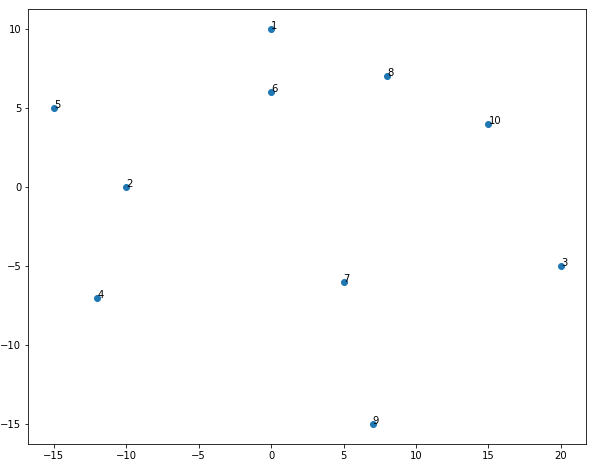
\includegraphics[]{resources/KD_points.PNG}

\begin{conseil}
La première division se fait de façon verticale. Veillez à bien insérer les points dans l'ordre (point 1, point 2, etc..). Les nœuds se situant au même niveau devraient diviser l'espace selon le même axe.
\end{conseil}
\begin{solution}
    Voici le KD-Tree correspondant :\\
    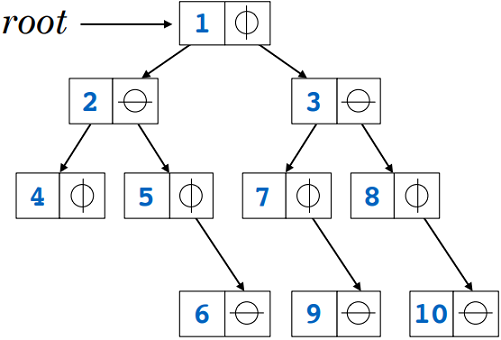
\includegraphics[]{resources/Kd-tree.PNG}\\
    Et la division de l'espace qui en résulte :\\
    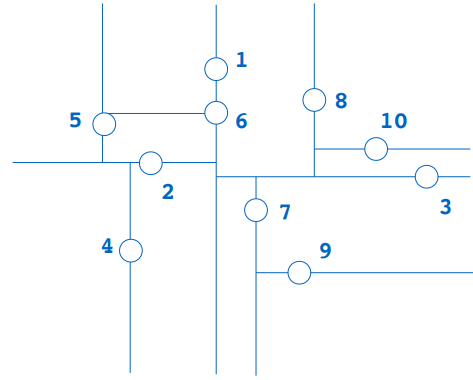
\includegraphics[]{resources/Division espace.PNG}
\end{solution}
\end{Exercice}

\newpage

\begin{Exercice}[15 minutes]\textbf{KD-Tree : Python}\\

L'objectif de cet exercice est d'écrire une fonction permettant d'ajouter un nœud à un KD-Tree. Les nœuds sont de la forme ((x,y), enfant à gauche, enfant à droite), x et y étant les coordonnées du nœud considéré. Chaque enfant peut être soit un nœud ou une feuille. Complétez le code contenu dans le fichier \lstinline{Question5.py}.\\

\begin{conseil}

% Veuillez vous référer aux pages 15 et 16 du cours de cette semaine. Ces pages expliquent le pseudo-code présent ci-dessous dont vous devez faire l'implémentation.

Voici le pseudo-code permettant d'ajouter un nœud à un KD-Tree :\\

ADD(node,point,cutaxis):\\
    \tabto{1cm}if node = NIL\\
        \tabto{2cm}node $\leftarrow$ Create-Node\\
        \tabto{2cm}node.point = point\\
        \tabto{2cm}return node\\
    \tabto{1cm}if point[cutaxis] $\leq$ node.point[cutaxis]\\
    \tabto{2cm} node.left = ADD(node.left, point, (cutaxis + 1) modulo k\\
    \tabto{1cm} else\\
    \tabto{2cm} node.right = ADD(node.right, point, (cutaxis+1) modulo k\\
    \tabto{1cm} return node\\
    
    Si votre réponse est correcte, votre programme devrait afficher : \lstinline{[(0, 10), [(-10, 0), None, None], None]}.\\
    Pour rappel, en Python, \lstinline{NIL} correspond à \lstinline{None}. \lstinline{Create-Node} permet de créer un nouveau nœud, vous pouvez vous inspirer de la structure de \lstinline{root} définie dans le fichier \lstinline{Question5.py}.
\end{conseil}

\begin{solution}
\lstinputlisting[language = python]{solutions/Question5_solution.py}

Si la coordonnée du point à ajouter est inférieure à celle du nœud selon l'axe de découpe en considération, alors le point doit se trouver dans le sous-arbre de gauche. Par convention, le nœud de gauche correspond dans la liste [(x,y), nœud de gauche, nœud de droite] à l'indice 1, par conséquent, on appelle la fonction de façon récursive pour ajouter le point, mais cette fois-ci en partant d'un cran plus bas dans l'arbre. Cela se répète jusqu'à ce qu'on ait atteint les feuilles et qu'un nouveau nœud doive être créé.

\end{solution}
\end{Exercice}

\newpage

\section{ Quad-Tree}
\begin{Exercice}[10 minutes]\textbf{Une mise en train : Papier}\\

Encodez les images ci-dessous dans un Quad-Tree.\\

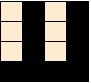
\includegraphics[]{resources/Quad-Tree 1.PNG}\\
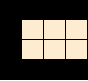
\includegraphics[]{resources/Quad-Tree 2.PNG}

\begin{conseil}
   Pour réussir cet exercice vous devez diviser chaque nœud en 4 sous-espaces (le plus petit sous-espace étant un carré) de taille égale, et ce autant de fois que nécessaire. La branche la plus à gauche correspond au quadrant \lstinline{NW} puis en allant de gauche à droite : \lstinline{NE, SW, SE}. \\
    
    \textbf{Indice :} Votre arbre devrait avoir une profondeur de 2 et disposer de 16 feuilles.
\end{conseil}
\begin{solution}
Image 1 :\\
    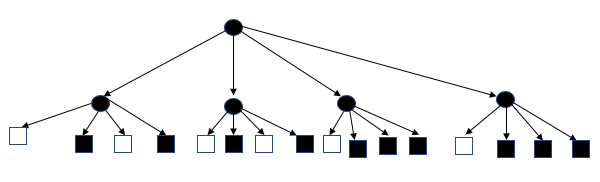
\includegraphics[scale=0.65]{solutions/Quad-Tree 1 solution.PNG}\\
    
Image 2: \\
    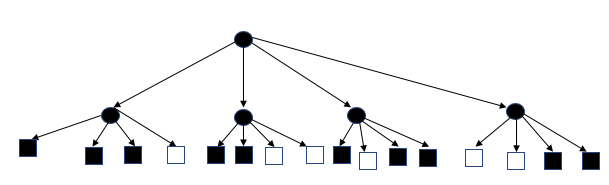
\includegraphics[scale=0.65]{solutions/Quad-Tree 2 solution.PNG}
\end{solution}
\end{Exercice}
\begin{Exercice}[10 minutes]\textbf{Une mission capitale : Papier \optionnel}\\

Récemment embauché par la CIA, vous êtes à la recherche d'un individu se cachant dans une des villes suivantes : Bleu, Orange, Noir, Gris, Vert et Jaune. Votre mission, si vous l'acceptez, est de créer un Quad-Tree qui vous permettra de géolocaliser le criminel de façon efficace. Vous trouverez ci-dessous une carte de villes. Créez le Quad-Tree et rétablissez la justice.\\

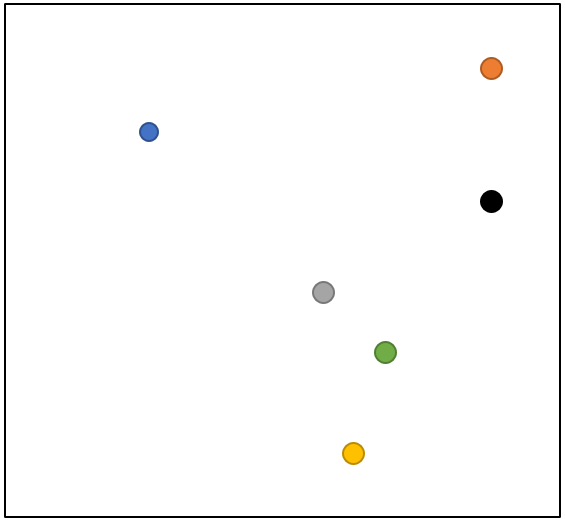
\includegraphics[]{resources/Quad-Tree 3.PNG}
\begin{conseil}
    Commencez par diviser la carte de la ville de façon adéquate puis construisez le graphe.\\
    
    \textbf{Remarque: }Les différentes branches de l'arbre n'auront pas toutes la même profondeur.
\end{conseil}
\begin{solution}
    Voici la division de la carte qui permet de construire le Quad-Tree :\\
    
    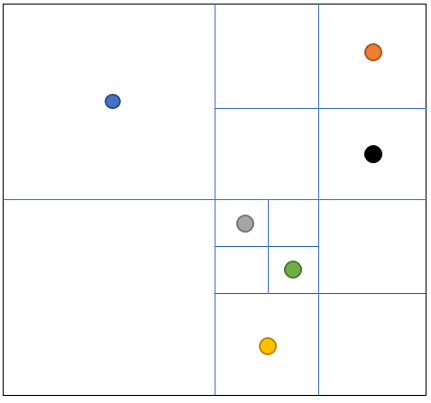
\includegraphics[]{solutions/Quad-Tree 3 solution 1.PNG}\\
    
    Le Quad-Tree qui en résulte :\\
    
    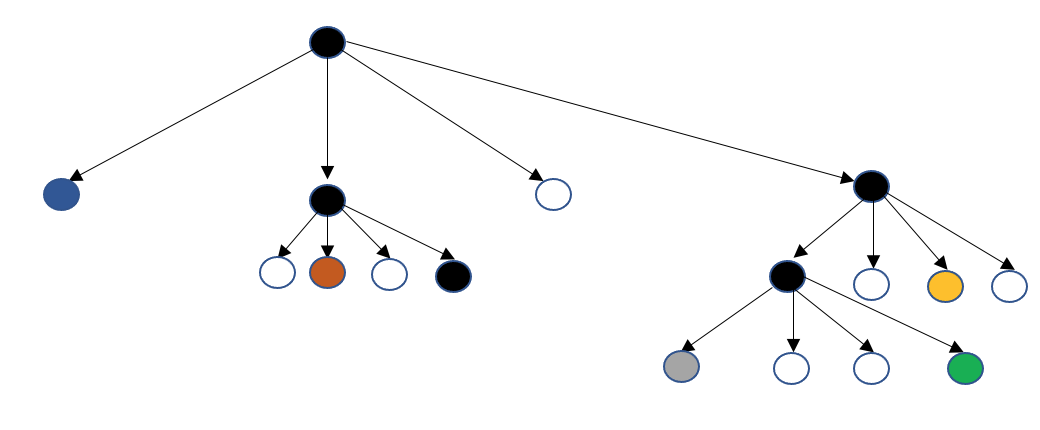
\includegraphics[scale=0.65]{solutions/Quad-Tree 3 solution 2.1.png}\\
    
    Note : Un rond blanc correspond à un quadrant vide.
    
\end{solution}
\end{Exercice}

\end{document}
